% Options for packages loaded elsewhere
\PassOptionsToPackage{unicode}{hyperref}
\PassOptionsToPackage{hyphens}{url}
%
\documentclass[
  english,
  man]{apa6}
\usepackage{lmodern}
\usepackage{amsmath}
\usepackage{ifxetex,ifluatex}
\ifnum 0\ifxetex 1\fi\ifluatex 1\fi=0 % if pdftex
  \usepackage[T1]{fontenc}
  \usepackage[utf8]{inputenc}
  \usepackage{textcomp} % provide euro and other symbols
  \usepackage{amssymb}
\else % if luatex or xetex
  \usepackage{unicode-math}
  \defaultfontfeatures{Scale=MatchLowercase}
  \defaultfontfeatures[\rmfamily]{Ligatures=TeX,Scale=1}
\fi
% Use upquote if available, for straight quotes in verbatim environments
\IfFileExists{upquote.sty}{\usepackage{upquote}}{}
\IfFileExists{microtype.sty}{% use microtype if available
  \usepackage[]{microtype}
  \UseMicrotypeSet[protrusion]{basicmath} % disable protrusion for tt fonts
}{}
\makeatletter
\@ifundefined{KOMAClassName}{% if non-KOMA class
  \IfFileExists{parskip.sty}{%
    \usepackage{parskip}
  }{% else
    \setlength{\parindent}{0pt}
    \setlength{\parskip}{6pt plus 2pt minus 1pt}}
}{% if KOMA class
  \KOMAoptions{parskip=half}}
\makeatother
\usepackage{xcolor}
\IfFileExists{xurl.sty}{\usepackage{xurl}}{} % add URL line breaks if available
\IfFileExists{bookmark.sty}{\usepackage{bookmark}}{\usepackage{hyperref}}
\hypersetup{
  pdftitle={Relationship between social capital and election results},
  pdfauthor={Anisha Babu1, Hyeonjin Cha1, Diana DeWald1, \& Murat Kezer1},
  pdflang={en-EN},
  pdfkeywords={keywords},
  hidelinks,
  pdfcreator={LaTeX via pandoc}}
\urlstyle{same} % disable monospaced font for URLs
\usepackage{graphicx}
\makeatletter
\def\maxwidth{\ifdim\Gin@nat@width>\linewidth\linewidth\else\Gin@nat@width\fi}
\def\maxheight{\ifdim\Gin@nat@height>\textheight\textheight\else\Gin@nat@height\fi}
\makeatother
% Scale images if necessary, so that they will not overflow the page
% margins by default, and it is still possible to overwrite the defaults
% using explicit options in \includegraphics[width, height, ...]{}
\setkeys{Gin}{width=\maxwidth,height=\maxheight,keepaspectratio}
% Set default figure placement to htbp
\makeatletter
\def\fps@figure{htbp}
\makeatother
\setlength{\emergencystretch}{3em} % prevent overfull lines
\providecommand{\tightlist}{%
  \setlength{\itemsep}{0pt}\setlength{\parskip}{0pt}}
\setcounter{secnumdepth}{-\maxdimen} % remove section numbering
% Make \paragraph and \subparagraph free-standing
\ifx\paragraph\undefined\else
  \let\oldparagraph\paragraph
  \renewcommand{\paragraph}[1]{\oldparagraph{#1}\mbox{}}
\fi
\ifx\subparagraph\undefined\else
  \let\oldsubparagraph\subparagraph
  \renewcommand{\subparagraph}[1]{\oldsubparagraph{#1}\mbox{}}
\fi
% Manuscript styling
\usepackage{upgreek}
\captionsetup{font=singlespacing,justification=justified}

% Table formatting
\usepackage{longtable}
\usepackage{lscape}
% \usepackage[counterclockwise]{rotating}   % Landscape page setup for large tables
\usepackage{multirow}		% Table styling
\usepackage{tabularx}		% Control Column width
\usepackage[flushleft]{threeparttable}	% Allows for three part tables with a specified notes section
\usepackage{threeparttablex}            % Lets threeparttable work with longtable

% Create new environments so endfloat can handle them
% \newenvironment{ltable}
%   {\begin{landscape}\begin{center}\begin{threeparttable}}
%   {\end{threeparttable}\end{center}\end{landscape}}
\newenvironment{lltable}{\begin{landscape}\begin{center}\begin{ThreePartTable}}{\end{ThreePartTable}\end{center}\end{landscape}}

% Enables adjusting longtable caption width to table width
% Solution found at http://golatex.de/longtable-mit-caption-so-breit-wie-die-tabelle-t15767.html
\makeatletter
\newcommand\LastLTentrywidth{1em}
\newlength\longtablewidth
\setlength{\longtablewidth}{1in}
\newcommand{\getlongtablewidth}{\begingroup \ifcsname LT@\roman{LT@tables}\endcsname \global\longtablewidth=0pt \renewcommand{\LT@entry}[2]{\global\advance\longtablewidth by ##2\relax\gdef\LastLTentrywidth{##2}}\@nameuse{LT@\roman{LT@tables}} \fi \endgroup}

% \setlength{\parindent}{0.5in}
% \setlength{\parskip}{0pt plus 0pt minus 0pt}

% \usepackage{etoolbox}
\makeatletter
\patchcmd{\HyOrg@maketitle}
  {\section{\normalfont\normalsize\abstractname}}
  {\section*{\normalfont\normalsize\abstractname}}
  {}{\typeout{Failed to patch abstract.}}
\patchcmd{\HyOrg@maketitle}
  {\section{\protect\normalfont{\@title}}}
  {\section*{\protect\normalfont{\@title}}}
  {}{\typeout{Failed to patch title.}}
\makeatother
\shorttitle{Title}
\keywords{keywords\newline\indent Word count: X}
\DeclareDelayedFloatFlavor{ThreePartTable}{table}
\DeclareDelayedFloatFlavor{lltable}{table}
\DeclareDelayedFloatFlavor*{longtable}{table}
\makeatletter
\renewcommand{\efloat@iwrite}[1]{\immediate\expandafter\protected@write\csname efloat@post#1\endcsname{}}
\makeatother
\usepackage{csquotes}
\ifxetex
  % Load polyglossia as late as possible: uses bidi with RTL langages (e.g. Hebrew, Arabic)
  \usepackage{polyglossia}
  \setmainlanguage[]{english}
\else
  \usepackage[shorthands=off,main=english]{babel}
\fi
\ifluatex
  \usepackage{selnolig}  % disable illegal ligatures
\fi
\usepackage[]{biblatex}
\addbibresource{r-references.bib}
\newlength{\cslhangindent}
\setlength{\cslhangindent}{1.5em}
\newlength{\csllabelwidth}
\setlength{\csllabelwidth}{3em}
\newenvironment{CSLReferences}[3] % #1 hanging-ident, #2 entry spacing
 {% don't indent paragraphs
  \setlength{\parindent}{0pt}
  % turn on hanging indent if param 1 is 1
  \ifodd #1 \everypar{\setlength{\hangindent}{\cslhangindent}}\ignorespaces\fi
  % set entry spacing
  \ifnum #2 > 0
  \setlength{\parskip}{#2\baselineskip}
  \fi
 }%
 {}
\usepackage{calc} % for \widthof, \maxof
\newcommand{\CSLBlock}[1]{#1\hfill\break}
\newcommand{\CSLLeftMargin}[1]{\parbox[t]{\maxof{\widthof{#1}}{\csllabelwidth}}{#1}}
\newcommand{\CSLRightInline}[1]{\parbox[t]{\linewidth}{#1}}
\newcommand{\CSLIndent}[1]{\hspace{\cslhangindent}#1}

\title{Relationship between social capital and election results}
\author{Anisha Babu\textsuperscript{1}, Hyeonjin Cha\textsuperscript{1}, Diana DeWald\textsuperscript{1}, \& Murat Kezer\textsuperscript{1}}
\date{}


\authornote{

Add complete departmental affiliations for each author here. Each new line herein must be indented, like this line.
Enter author note here.

The authors made the following contributions. Anisha Babu: Conceptualization, Data Analysis, Writing - Original Draft Preparation, Writing - Review \& Editing; Hyeonjin Cha: Conceptualization, Data Analysis, Writing - Original Draft Preparation, Writing - Review \& Editing; Diana DeWald: Conceptualization, Data Analysis, Writing - Original Draft Preparation, Writing - Review \& Editing; Murat Kezer: Conceptualization, Data Analysis, Writing - Original Draft Preparation, Writing - Review \& Editing.

}

\affiliation{\vspace{0.5cm}\textsuperscript{1} University of Oregon}

\abstract{
One or two sentences providing a \textbf{basic introduction} to the field, comprehensible to a scientist in any discipline.

Two to three sentences of \textbf{more detailed background}, comprehensible to scientists in related disciplines.

One sentence clearly stating the \textbf{general problem} being addressed by this particular study.

One sentence summarizing the main result (with the words ``\textbf{here we show}'' or their equivalent).

Two or three sentences explaining what the \textbf{main result} reveals in direct comparison to what was thought to be the case previously, or how the main result adds to previous knowledge.

One or two sentences to put the results into a more \textbf{general context}.

Two or three sentences to provide a \textbf{broader perspective}, readily comprehensible to a scientist in any discipline.
}



\begin{document}
\maketitle

\hypertarget{introduction}{%
\section{Introduction}\label{introduction}}

Social science literature has extensively examined the relationship between social capital and politics (e.g.~Morales \& Guigni, 2016; Jottier \& Heyndels, 2012; La Due Lake \& Huckfeldt, 1998). However, relatively little is known on the impact of social capital election results.

\hypertarget{methods}{%
\section{Methods}\label{methods}}

We report how we determined our sample size, all data exclusions (if any), all manipulations, and all measures in the study.

\hypertarget{data}{%
\subsection{Data}\label{data}}

\begin{itemize}
\tightlist
\item
  County Presidential Election Returns 2000-2016 (MIT Election Data and Science Lab, 2018)

  \begin{itemize}
  \tightlist
  \item
    County level returns for presidential elections from 2000 to 2016
  \item
    Election results across the years in one dataset \& in tidy format
  \end{itemize}
\item
  The production of social capital in US counties (Rupasingha, Goetz, \& Freshwater, 2006, with updates)

  \begin{itemize}
  \tightlist
  \item
    County level count of various establishments defined by NAICS code
  \item
    Different variables measured across years; new dataset for each year
  \end{itemize}
\end{itemize}

\hypertarget{data-preparation}{%
\subsection{Data Preparation}\label{data-preparation}}

\hypertarget{load-data-and-clean-names}{%
\subsubsection{Load data and clean names}\label{load-data-and-clean-names}}

We first load the datasets and clean the variable names.

\hypertarget{clean-data}{%
\subsubsection{Clean data}\label{clean-data}}

\hypertarget{election-data}{%
\paragraph{Election data}\label{election-data}}

\begin{itemize}
\item
  We start with the election data as it is more comprehensive in terms of the number of counties. First, we select the variables of interests. Then, we select the election year (i.e., 2000, 2008, 2012, 2016) that we will match with social capital data.
\item
  The name of the year variable is changed in a way that shows it is the year of election (so that it is not mixed with the same year variable in social capital data).
\item
  We create new datasets for each presidential election we are interested in. These will be later merged with corresponding social capital data.
\end{itemize}

\hypertarget{social-capital-data}{%
\paragraph{Social capital data}\label{social-capital-data}}

\begin{itemize}
\item
  For each social capital dataset (i.e., 1997, 2005, 2009, 2014), we first add state code for some counties that do not readily contain that information. Then, we create two variables out of the area name such that we have different variables for county names and state codes.
\item
  We select the relevant variables and clean the variable names.
\item
  We create a year variable indicating when the data were collected.
\item
  Finally, we reorder variables so that the order of the variables is the same across datasets. This will be useful when we want to merge social capital data across year so that we can get descriptive statistics for each year simultaneously and that we can visualize the changes across years in social capital.
\end{itemize}

\hypertarget{merge-datasets}{%
\subsubsection{Merge Datasets}\label{merge-datasets}}

\begin{itemize}
\item
  First, we merge social capital data across years for reasons explained above, and call it \texttt{s\_capital}.
\item
  Next, we merge corresponding election and social capital data for 4 time points. \textbf{In doing so,} we keep the rows that exist in both election and social capital data. For instance, if we do not have the election information for a county, we do not include it in the merged dataset even if we have that county's social capital data. These datasets are called \texttt{df\_year}. \emph{Year} denotes the year of election. Also, we remove the duplicate variables (i.e., state and county names) and fix the names. We did not remove them earlier because we first wanted to merge the social capital data with all the variables.
\item
  Finally, we merge all election and social capital data in the same dataset (i.e., \texttt{df}). In addition, we created another dataset using \texttt{pivot\_wider()} to have variables for the candidate votes per political party. Then, we removed the intermediate objects (i.e., all data frames except for \texttt{df} and \texttt{df\_wide}).
\end{itemize}

\hypertarget{data-analysis}{%
\subsection{Data analysis}\label{data-analysis}}

\begin{verbatim}
##                  bowl        civic          golf         relig        sport
## bowl       1.00000000  0.163331564  0.1843690062  1.754235e-01 -0.011262877
## civic      0.16333156  1.000000000  0.1658962995  2.547000e-01 -0.003264050
## golf       0.18436901  0.165896299  1.0000000000  3.491323e-01 -0.021985208
## relig      0.17542352  0.254699957  0.3491322736  1.000000e+00  0.002806421
## sport     -0.01126288 -0.003264050 -0.0219852075  2.806421e-03  1.000000000
## pol       -0.02966700  0.001966347 -0.0334108615 -9.423555e-05  0.012883481
## prof      -0.01392921  0.076733734 -0.0417492547 -3.323368e-02  0.021631055
## bus        0.09723730  0.140544743  0.1370127533  3.110755e-01 -0.020948989
## labor      0.01396846  0.127298046 -0.0318697416 -4.609051e-02  0.017101150
## respn      0.04573144  0.033975898  0.0008135967 -8.286148e-03 -0.004274877
## pvote      0.08361274  0.095880533  0.1007224264  4.908534e-02  0.028533722
## pop       -0.06101167 -0.070326839 -0.1026103152 -2.262784e-01  0.023425173
## nccs       0.22185326  0.347937372  0.2808439095  3.743616e-01  0.017981863
## assn       0.29451849  0.484150132  0.4950591900  9.183900e-01  0.023813113
## demmargin -0.09156467 -0.037419358 -0.1379312816 -3.337933e-01  0.024754801
##                     pol        prof         bus         labor         respn
## bowl      -2.966700e-02 -0.01392921  0.09723730  0.0139684639  0.0457314391
## civic      1.966347e-03  0.07673373  0.14054474  0.1272980463  0.0339758984
## golf      -3.341086e-02 -0.04174925  0.13701275 -0.0318697416  0.0008135967
## relig     -9.423555e-05 -0.03323368  0.31107552 -0.0460905051 -0.0082861484
## sport      1.288348e-02  0.02163105 -0.02094899  0.0171011497 -0.0042748774
## pol        1.000000e+00  0.20178507  0.08837989  0.0511035445 -0.0353395859
## prof       2.017851e-01  1.00000000  0.16314793  0.1102856692  0.0756318706
## bus        8.837989e-02  0.16314793  1.00000000 -0.0188081662 -0.1678024962
## labor      5.110354e-02  0.11028567 -0.01880817  1.0000000000  0.1920688496
## respn     -3.533959e-02  0.07563187 -0.16780250  0.1920688496  1.0000000000
## pvote      4.581321e-02  0.04152891  0.07735125 -0.0036691656  0.1131580514
## pop        4.668483e-02  0.08947146 -0.09489972  0.0586595869  0.1039281594
## nccs       8.661840e-02  0.13549486  0.32688972 -0.0002338711 -0.1209083839
## assn       6.319277e-02  0.09392249  0.47070855  0.0830621339  0.0133341334
## demmargin  8.501235e-02  0.18630848 -0.09135165  0.1315740835  0.0595954442
##                  pvote         pop          nccs        assn   demmargin
## bowl       0.083612738 -0.06101167  0.2218532641  0.29451849 -0.09156467
## civic      0.095880533 -0.07032684  0.3479373723  0.48415013 -0.03741936
## golf       0.100722426 -0.10261032  0.2808439095  0.49505919 -0.13793128
## relig      0.049085341 -0.22627840  0.3743615599  0.91838999 -0.33379330
## sport      0.028533722  0.02342517  0.0179818630  0.02381311  0.02475480
## pol        0.045813214  0.04668483  0.0866183961  0.06319277  0.08501235
## prof       0.041528912  0.08947146  0.1354948632  0.09392249  0.18630848
## bus        0.077351254 -0.09489972  0.3268897173  0.47070855 -0.09135165
## labor     -0.003669166  0.05865959 -0.0002338711  0.08306213  0.13157408
## respn      0.113158051  0.10392816 -0.1209083839  0.01333413  0.05959544
## pvote      1.000000000  0.02826091  0.2303456902  0.11604985  0.10013568
## pop        0.028260911  1.00000000 -0.0958799517 -0.19781990  0.35179190
## nccs       0.230345690 -0.09587995  1.0000000000  0.49110261 -0.06627689
## assn       0.116049854 -0.19781990  0.4911026061  1.00000000 -0.25818469
## demmargin  0.100135681  0.35179190 -0.0662768883 -0.25818469  1.00000000
\end{verbatim}

\begin{verbatim}
## 
## Call:
## lm(formula = demmargin ~ 1 + bowl + civic + golf + relig + sport + 
##     pol + prof + bus + labor + pvote + respn + pop, data = df_anal_2016)
## 
## Residuals:
##      Min       1Q   Median       3Q      Max 
## -1.90456 -0.18538 -0.04293  0.15323  1.21563 
## 
## Coefficients:
##               Estimate Std. Error t value Pr(>|t|)    
## (Intercept) -4.604e-01  4.802e-02  -9.588  < 2e-16 ***
## bowl        -2.034e-01  9.204e-02  -2.210   0.0272 *  
## civic        6.436e-02  3.853e-02   1.671   0.0949 .  
## golf        -4.419e-02  4.695e-02  -0.941   0.3467    
## relig       -1.583e-01  1.110e-02 -14.253  < 2e-16 ***
## sport        1.861e-01  2.800e-01   0.665   0.5064    
## pol          4.993e-01  2.240e-01   2.229   0.0259 *  
## prof         1.165e+00  1.454e-01   8.011 1.60e-15 ***
## bus         -4.153e-02  4.610e-02  -0.901   0.3677    
## labor        4.958e-01  9.433e-02   5.256 1.58e-07 ***
## pvote        3.632e-01  5.692e-02   6.381 2.02e-10 ***
## respn       -2.638e-02  4.800e-02  -0.550   0.5826    
## pop          2.653e-07  1.607e-08  16.504  < 2e-16 ***
## ---
## Signif. codes:  0 '***' 0.001 '**' 0.01 '*' 0.05 '.' 0.1 ' ' 1
## 
## Residual standard error: 0.283 on 3102 degrees of freedom
## Multiple R-squared:  0.2362, Adjusted R-squared:  0.2333 
## F-statistic: 79.94 on 12 and 3102 DF,  p-value: < 2.2e-16
\end{verbatim}

\begin{verbatim}
## # A tibble: 51 x 6
##    state_po     n m_totalvotes sd_totalvotes mean_pop   sd_pop
##    <chr>    <int>        <dbl>         <dbl>    <dbl>    <dbl>
##  1 AK           3        7036.          460.  103142.  170798.
##  2 AL         268       29724.        45394.   69187.  101303.
##  3 AR         300       14026.        21417.   37486.   53831.
##  4 AZ          60      145927.       330585.  394133.  889795.
##  5 CA         232      223051.       465584.  620980. 1387279.
##  6 CO         253       37272.        75235.   74612.  150559.
##  7 CT          32      196409.       151721.  437902.  347809.
##  8 DC           4      268195.        47994.  596734    43662.
##  9 DE          12      133073.        85452.  285361.  178905.
## 10 FL         267      118431.       173570.  260031.  415642.
## # ... with 41 more rows
\end{verbatim}

\begin{verbatim}
## # A tibble: 13 x 5
## # Groups:   year_elctn [4]
##    year_elctn party     n m_candidatevotes sd_candidatevotes
##         <int> <fct> <int>            <dbl>             <dbl>
##  1       2000 Dem    3107           16218.            57150.
##  2       2000 Green  3107              NA                NA 
##  3       2000 Rep    3107           16049.            38632.
##  4       2000 <NA>   3107             339.              954.
##  5       2008 Dem    3108           22157.            76972.
##  6       2008 Rep    3108           19167.            44840.
##  7       2008 <NA>   3108             577.             1848.
##  8       2012 Dem    3108           20974.            73998.
##  9       2012 Rep    3108           19409.            44596.
## 10       2012 <NA>   3108             838.             2952.
## 11       2016 Dem    3115           21071.            80496.
## 12       2016 Rep    3115           20160.            43157.
## 13       2016 <NA>   3115            2449.             7509.
\end{verbatim}

\begin{verbatim}
## # A tibble: 36 x 7
## # Groups:   county, relig, civic, labor, democrat [36]
##    county    relig civic labor democrat republican voter_turnout
##    <chr>     <dbl> <dbl> <dbl>    <int>      <int>         <dbl>
##  1 Baker        11     5     1     2195       5618          64.8
##  2 Benton       50    13     3    19444      15825          63.3
##  3 Clackamas   184    32    13    76421      77539          62.8
##  4 Clatsop      35    12     7     8296       6950          60.8
##  5 Columbia     29     5     3    10331       9369          62.0
##  6 Coos         40     9     7    11610      15626          59.9
##  7 Crook        14     3     0     2474       5363          59.5
##  8 Curry        13     1     1     4090       6551          66.8
##  9 Deschutes    62    29     8    22061      32132          63.7
## 10 Douglas      77    12     4    14193      30294          59.6
## # ... with 26 more rows
\end{verbatim}

\begin{verbatim}
## # A tibble: 36 x 7
## # Groups:   county, relig, civic, labor, democrat [36]
##    county    relig civic labor democrat republican voter_turnout
##    <chr>     <dbl> <dbl> <dbl>    <int>      <int>         <dbl>
##  1 Baker        19     5     2     2805       5650            70
##  2 Benton       60    15     7    29901      15264            73
##  3 Clackamas   206    20    15   103476      83595            71
##  4 Clatsop      31    12     5    10701       7192            68
##  5 Columbia     31     4     1    13390      10413            71
##  6 Coos         46     8     7    14401      15354            65
##  7 Crook        15     4     0     3632       6371            62
##  8 Curry        17     2     0     5230       6646            70
##  9 Deschutes    81    22     5    38819      39064            71
## 10 Douglas      81     7     4    20298      30919            68
## # ... with 26 more rows
\end{verbatim}

\begin{verbatim}
## # A tibble: 36 x 7
## # Groups:   county, relig, civic, labor, democrat [36]
##    county    relig civic labor democrat republican voter_turnout
##    <chr>     <dbl> <dbl> <dbl>    <int>      <int>         <dbl>
##  1 Baker        16     5     1     2369       5702          68.2
##  2 Benton       60    14     5    27776      14991          69.3
##  3 Clackamas   197    21    15    95493      88592          64.8
##  4 Clatsop      28    10     5     9861       7249          62.4
##  5 Columbia     32     3     2    12004      10772          64.6
##  6 Coos         53     7     6    12845      14673          60.1
##  7 Crook        17     4     0     3104       6790          57.9
##  8 Curry        14     1     0     4625       6598          67.9
##  9 Deschutes    95    19     8    36961      42463          64.6
## 10 Douglas      87     8     4    17145      30776          63.7
## # ... with 26 more rows
\end{verbatim}

\begin{verbatim}
## # A tibble: 36 x 7
## # Groups:   county, relig, civic, labor, democrat [36]
##    county    relig civic labor democrat republican voter_turnout
##    <chr>     <dbl> <dbl> <dbl>    <int>      <int>         <dbl>
##  1 Baker        20     8     1     1797       6218          83.1
##  2 Benton       66    13     5    29193      13445          85.7
##  3 Clackamas   215    20    18   102095      88392          82.5
##  4 Clatsop      31    11     3     9252       8138          82.2
##  5 Columbia     26     4     2    10167      13217          82.2
##  6 Coos         53     7     5    10448      17865          82.2
##  7 Crook        20     3     0     2637       8511          83.2
##  8 Curry        15     1     0     4300       7212          84.3
##  9 Deschutes    92    22     7    42444      45692          84.1
## 10 Douglas      90     7     3    14096      34582          79.6
## # ... with 26 more rows
\end{verbatim}

\begin{table}

\caption{(\#tab:descriptives tables)<b>Table 1</b><br /> <i>A summary table for total votes and population by state.</i>}
\centering
\begin{tabular}[t]{c|c|c|c|c|c}
\hline
\multicolumn{2}{c|}{ } & \multicolumn{2}{c|}{Total Votes} & \multicolumn{2}{c}{Population} \\
\cline{3-4} \cline{5-6}
Sate & N & M & SD & M & SD\\
\hline
AK & 3 & 7036 & 460 & 103142 & 170798\\
\hline
AL & 268 & 29724 & 45394 & 69187 & 101303\\
\hline
AR & 300 & 14026 & 21417 & 37486 & 53831\\
\hline
AZ & 60 & 145927 & 330585 & 394133 & 889795\\
\hline
CA & 232 & 223051 & 465584 & 620980 & 1387279\\
\hline
CO & 253 & 37272 & 75235 & 74612 & 150559\\
\hline
CT & 32 & 196409 & 151721 & 437902 & 347809\\
\hline
DC & 4 & 268195 & 47994 & 596734 & 43662\\
\hline
DE & 12 & 133073 & 85452 & 285361 & 178905\\
\hline
FL & 267 & 118431 & 173570 & 260031 & 415642\\
\hline
GA & 636 & 22857 & 51210 & 57121 & 120420\\
\hline
HI & 4 & 107234 & 120109 & 355042 & 427919\\
\hline
IA & 396 & 15153 & 26357 & 30298 & 50767\\
\hline
ID & 176 & 14201 & 27837 & 33216 & 61206\\
\hline
IL & 408 & 51632 & 207620 & 123712 & 528335\\
\hline
IN & 368 & 28016 & 45752 & 68726 & 113969\\
\hline
KS & 420 & 11068 & 32305 & 26466 & 70945\\
\hline
KY & 480 & 14775 & 33166 & 35136 & 71897\\
\hline
LA & 256 & 30265 & 40734 & 70853 & 97369\\
\hline
MA & 56 & 218333 & 190389 & 462537 & 397378\\
\hline
MD & 96 & 105686 & 125998 & 233911 & 281901\\
\hline
ME & 64 & 44329 & 39811 & 81772 & 69901\\
\hline
MI & 332 & 56520 & 122899 & 119512 & 266186\\
\hline
MN & 348 & 32271 & 79906 & 59257 & 141434\\
\hline
MO & 460 & 22676 & 57042 & 50644 & 121028\\
\hline
MS & 328 & 14558 & 15660 & 35473 & 40323\\
\hline
MT & 224 & 8429 & 14226 & 17130 & 28610\\
\hline
NC & 400 & 41172 & 66022 & 89380 & 130861\\
\hline
ND & 212 & 6001 & 11857 & 12740 & 24158\\
\hline
NE & 372 & 8432 & 26489 & 19203 & 59844\\
\hline
NH & 40 & 68382 & 60667 & 128300 & 114741\\
\hline
NJ & 84 & 173096 & 101198 & 411491 & 246050\\
\hline
NM & 132 & 22809 & 45608 & 59314 & 109938\\
\hline
NV & 68 & 54664 & 153035 & 142929 & 417902\\
\hline
NY & 248 & 117671 & 180993 & 309859 & 525415\\
\hline
OH & 352 & 61025 & 101857 & 130303 & 213470\\
\hline
OK & 308 & 17808 & 40041 & 47139 & 103956\\
\hline
OR & 144 & 49670 & 76632 & 102065 & 154506\\
\hline
PA & 268 & 84879 & 127302 & 187084 & 266098\\
\hline
RI & 20 & 89501 & 79885 & 210091 & 216763\\
\hline
SC & 184 & 40065 & 44227 & 95374 & 101465\\
\hline
SD & 264 & 5409 & 10619 & 12046 & 23307\\
\hline
TN & 380 & 25376 & 49406 & 64063 & 122210\\
\hline
TX & 1016 & 30953 & 105483 & 92814 & 333875\\
\hline
UT & 116 & 33379 & 74041 & 88323 & 198237\\
\hline
VA & 535 & 26730 & 53718 & 57289 & 111708\\
\hline
VT & 56 & 22031 & 18096 & 44108 & 34787\\
\hline
WA & 156 & 76026 & 158419 & 164504 & 328036\\
\hline
WI & 288 & 40379 & 67838 & 77226 & 129823\\
\hline
WV & 220 & 12478 & 12682 & 33346 & 32720\\
\hline
WY & 92 & 10645 & 9351 & 23345 & 21584\\
\hline
\multicolumn{6}{l}{\rule{0pt}{1em}\textit{Note: } N = number of counties with recorded data per the four time points (2000, 2008, 2012, 2016).}\\
\end{tabular}
\end{table}

\begin{table}

\caption{(\#tab:descriptives tables)<b>Table 2</b><br /> <i>A summary table for votes by candidate and year of election.</i>}
\centering
\begin{tabular}[t]{c|c|c|c|c}
\hline
Year & Party & N & Mean Candidate Votes & SD Candidate Votes\\
\hline
2000 & Dem & 3107 & 16218 & 57150\\
\hline
2000 & Green & 3107 & -- & --\\
\hline
2000 & Rep & 3107 & 16049 & 38632\\
\hline
2000 & -- & 3107 & 339 & 954\\
\hline
2008 & Dem & 3108 & 22157 & 76972\\
\hline
2008 & Rep & 3108 & 19167 & 44840\\
\hline
2008 & -- & 3108 & 577 & 1848\\
\hline
2012 & Dem & 3108 & 20974 & 73998\\
\hline
2012 & Rep & 3108 & 19409 & 44596\\
\hline
2012 & -- & 3108 & 838 & 2952\\
\hline
2016 & Dem & 3115 & 21071 & 80496\\
\hline
2016 & Rep & 3115 & 20160 & 43157\\
\hline
2016 & -- & 3115 & 2449 & 7509\\
\hline
\multicolumn{5}{l}{\rule{0pt}{1em}\textit{Note: } N = total number of counties in the US reporting data.}\\
\end{tabular}
\end{table}

\begin{table}

\caption{(\#tab:descriptives tables)<b>Table 3</b><br /> <i>A summary table for the year 2000: Selected social capital and voting behavior in Oregon counties.</i>}
\centering
\begin{tabular}[t]{c|c|c|c|c|c|c}
\hline
County & Religious Organizations & Civic Associations & Labor Organizations & Votes Democrat & Votes Republican & Voter Turnout (\%)\\
\hline
Baker & 11 & 5 & 1 & 2195 & 5618 & 64.8\\
\hline
Benton & 50 & 13 & 3 & 19444 & 15825 & 63.3\\
\hline
Clackamas & 184 & 32 & 13 & 76421 & 77539 & 62.8\\
\hline
Clatsop & 35 & 12 & 7 & 8296 & 6950 & 60.8\\
\hline
Columbia & 29 & 5 & 3 & 10331 & 9369 & 62.0\\
\hline
Coos & 40 & 9 & 7 & 11610 & 15626 & 59.9\\
\hline
Crook & 14 & 3 & 0 & 2474 & 5363 & 59.5\\
\hline
Curry & 13 & 1 & 1 & 4090 & 6551 & 66.8\\
\hline
Deschutes & 62 & 29 & 8 & 22061 & 32132 & 63.7\\
\hline
Douglas & 77 & 12 & 4 & 14193 & 30294 & 59.6\\
\hline
Gilliam & 1 & 1 & 0 & 359 & 679 & 74.1\\
\hline
Grant & 4 & 1 & 0 & 589 & 3078 & 67.5\\
\hline
Harney & 7 & 2 & 0 & 766 & 2799 & 70.1\\
\hline
Hood River & 15 & 5 & 2 & 4072 & 3721 & 55.9\\
\hline
Jackson & 90 & 26 & 14 & 33153 & 46052 & 60.3\\
\hline
Jefferson & 11 & 1 & 0 & 2681 & 3838 & 56.6\\
\hline
Josephine & 35 & 12 & 0 & 11864 & 22186 & 60.0\\
\hline
Klamath & 45 & 15 & 6 & 7541 & 18855 & 50.7\\
\hline
Lake & 6 & 2 & 0 & 707 & 2830 & 70.9\\
\hline
Lane & 184 & 51 & 30 & 78583 & 61578 & 62.9\\
\hline
Lincoln & 32 & 17 & 1 & 10861 & 8446 & 60.7\\
\hline
Linn & 84 & 21 & 14 & 16682 & 25359 & 57.0\\
\hline
Malheur & 22 & 3 & 0 & 2336 & 7624 & 52.5\\
\hline
Marion & 156 & 30 & 25 & 49430 & 57443 & 58.3\\
\hline
Morrow & 5 & 3 & 0 & 1197 & 2224 & 53.8\\
\hline
Multnomah & 386 & 92 & 103 & 188441 & 83677 & 58.0\\
\hline
Polk & 39 & 9 & 2 & 11921 & 14988 & 61.8\\
\hline
Sherman & 0 & 0 & 0 & 326 & 679 & 82.0\\
\hline
Tillamook & 22 & 5 & 1 & 5762 & 5775 & 62.8\\
\hline
Umatilla & 47 & 10 & 4 & 7809 & 14140 & 48.1\\
\hline
Union & 25 & 5 & 5 & 3577 & 7836 & 65.4\\
\hline
Wallowa & 4 & 3 & 0 & 836 & 3279 & 79.3\\
\hline
Wasco & 24 & 4 & 1 & 4616 & 5356 & 60.7\\
\hline
Washington & 171 & 29 & 21 & 90662 & 86091 & 58.7\\
\hline
Wheeler & 0 & 0 & 0 & 202 & 584 & 69.0\\
\hline
Yamhill & 62 & 5 & 2 & 14254 & 19193 & 58.3\\
\hline
\end{tabular}
\end{table}

\begin{table}

\caption{(\#tab:descriptives tables)<b>Table 4</b><br /> <i>A summary table for 2008: Selected social capital and voting behavior in Oregon counties.</i>}
\centering
\begin{tabular}[t]{c|c|c|c|c|c|c}
\hline
County & Religious Organizations & Civic Associations & Labor Organizations & Democrat & Republican & Voter Turnout (\%)\\
\hline
Baker & 19 & 5 & 2 & 2805 & 5650 & 70\\
\hline
Benton & 60 & 15 & 7 & 29901 & 15264 & 73\\
\hline
Clackamas & 206 & 20 & 15 & 103476 & 83595 & 71\\
\hline
Clatsop & 31 & 12 & 5 & 10701 & 7192 & 68\\
\hline
Columbia & 31 & 4 & 1 & 13390 & 10413 & 71\\
\hline
Coos & 46 & 8 & 7 & 14401 & 15354 & 65\\
\hline
Crook & 15 & 4 & 0 & 3632 & 6371 & 62\\
\hline
Curry & 17 & 2 & 0 & 5230 & 6646 & 70\\
\hline
Deschutes & 81 & 22 & 5 & 38819 & 39064 & 71\\
\hline
Douglas & 81 & 7 & 4 & 20298 & 30919 & 68\\
\hline
Gilliam & 1 & 1 & 0 & 430 & 648 & 78\\
\hline
Grant & 8 & 1 & 0 & 1006 & 2785 & 71\\
\hline
Harney & 6 & 1 & 0 & 950 & 2595 & 69\\
\hline
Hood River & 23 & 6 & 2 & 6302 & 3265 & 64\\
\hline
Jackson & 102 & 17 & 13 & 49090 & 49043 & 68\\
\hline
Jefferson & 13 & 4 & 1 & 3682 & 4402 & 57\\
\hline
Josephine & 47 & 12 & 2 & 17412 & 22973 & 67\\
\hline
Klamath & 51 & 13 & 5 & 9370 & 19113 & 64\\
\hline
Lake & 5 & 4 & 0 & 957 & 2638 & 68\\
\hline
Lane & 204 & 45 & 25 & 114037 & 63835 & 71\\
\hline
Lincoln & 30 & 11 & 1 & 14258 & 8791 & 67\\
\hline
Linn & 86 & 14 & 11 & 22163 & 28071 & 64\\
\hline
Malheur & 19 & 1 & 1 & 2949 & 7157 & 47\\
\hline
Marion & 183 & 24 & 28 & 61816 & 59059 & 58\\
\hline
Morrow & 9 & 2 & 0 & 1410 & 2509 & 51\\
\hline
Multnomah & 416 & 71 & 99 & 279696 & 75171 & 70\\
\hline
Polk & 50 & 9 & 1 & 17536 & 17714 & 68\\
\hline
Sherman & 4 & 0 & 0 & 385 & 634 & 84\\
\hline
Tillamook & 24 & 3 & 0 & 7072 & 5757 & 70\\
\hline
Umatilla & 51 & 10 & 3 & 9484 & 15254 & 50\\
\hline
Union & 29 & 4 & 5 & 4613 & 7581 & 72\\
\hline
Wallowa & 7 & 2 & 0 & 1492 & 2836 & 82\\
\hline
Wasco & 24 & 6 & 1 & 5906 & 5103 & 67\\
\hline
Washington & 209 & 31 & 9 & 141544 & 89185 & 64\\
\hline
Wheeler & 1 & 0 & 0 & 281 & 498 & 73\\
\hline
Yamhill & 70 & 4 & 3 & 20797 & 21390 & 62\\
\hline
\end{tabular}
\end{table}

\begin{table}

\caption{(\#tab:descriptives tables)<b>Table 5</b><br /> <i>A summary table for 2012: Selected social capital and voting behavior in Oregon counties.</i>}
\centering
\begin{tabular}[t]{c|c|c|c|c|c|c}
\hline
County & Religious Organizations & Civic Associations & Labor Organizations & Democrat & Republican & Voter Turnout (\%)\\
\hline
Baker & 16 & 5 & 1 & 2369 & 5702 & 68.2\\
\hline
Benton & 60 & 14 & 5 & 27776 & 14991 & 69.3\\
\hline
Clackamas & 197 & 21 & 15 & 95493 & 88592 & 64.8\\
\hline
Clatsop & 28 & 10 & 5 & 9861 & 7249 & 62.4\\
\hline
Columbia & 32 & 3 & 2 & 12004 & 10772 & 64.6\\
\hline
Coos & 53 & 7 & 6 & 12845 & 14673 & 60.1\\
\hline
Crook & 17 & 4 & 0 & 3104 & 6790 & 57.9\\
\hline
Curry & 14 & 1 & 0 & 4625 & 6598 & 67.9\\
\hline
Deschutes & 95 & 19 & 8 & 36961 & 42463 & 64.6\\
\hline
Douglas & 87 & 8 & 4 & 17145 & 30776 & 63.7\\
\hline
Gilliam & 1 & 1 & 0 & 371 & 639 & 76.4\\
\hline
Grant & 9 & 1 & 0 & 853 & 2926 & 70.3\\
\hline
Harney & 5 & 1 & 0 & 832 & 2607 & 70.1\\
\hline
Hood River & 22 & 5 & 1 & 6058 & 3429 & 61.4\\
\hline
Jackson & 104 & 17 & 14 & 44468 & 49020 & 64.0\\
\hline
Jefferson & 14 & 5 & 0 & 3301 & 4642 & 55.9\\
\hline
Josephine & 47 & 11 & 2 & 14953 & 23673 & 64.5\\
\hline
Klamath & 50 & 11 & 4 & 8302 & 18898 & 57.7\\
\hline
Lake & 6 & 4 & 0 & 770 & 2808 & 63.3\\
\hline
Lane & 202 & 39 & 26 & 102652 & 62509 & 66.0\\
\hline
Lincoln & 31 & 12 & 1 & 13401 & 8686 & 64.1\\
\hline
Linn & 87 & 14 & 10 & 20378 & 28944 & 59.0\\
\hline
Malheur & 19 & 2 & 2 & 2759 & 6851 & 45.3\\
\hline
Marion & 194 & 22 & 24 & 56376 & 60190 & 54.0\\
\hline
Morrow & 10 & 2 & 0 & 1202 & 2532 & 50.9\\
\hline
Multnomah & 413 & 67 & 96 & 274887 & 75302 & 66.2\\
\hline
Polk & 50 & 7 & 0 & 16292 & 17819 & 59.9\\
\hline
Sherman & 4 & 0 & 0 & 319 & 678 & 77.3\\
\hline
Tillamook & 24 & 4 & 0 & 6293 & 5684 & 66.8\\
\hline
Umatilla & 55 & 8 & 4 & 8584 & 15499 & 46.9\\
\hline
Union & 30 & 5 & 7 & 3973 & 7636 & 64.5\\
\hline
Wallowa & 6 & 2 & 0 & 1253 & 2804 & 80.7\\
\hline
Wasco & 23 & 5 & 1 & 5211 & 5229 & 62.1\\
\hline
Washington & 224 & 25 & 12 & 135291 & 93974 & 60.5\\
\hline
Wheeler & 0 & 0 & 0 & 266 & 545 & 73.1\\
\hline
Yamhill & 76 & 5 & 3 & 19260 & 22045 & 58.2\\
\hline
\end{tabular}
\end{table}

\begin{table}

\caption{(\#tab:descriptives tables)<b>Table 6</b><br /> <i>A summary table for 2016: Selected social capital and voting behavior in Oregon counties.</i>}
\centering
\begin{tabular}[t]{c|c|c|c|c|c|c}
\hline
County & Religious Organizations & Civic Associations & Labor Organizations & Democrat & Republican & Voter Turnout (\%)\\
\hline
Baker & 20 & 8 & 1 & 1797 & 6218 & 83.1\\
\hline
Benton & 66 & 13 & 5 & 29193 & 13445 & 85.7\\
\hline
Clackamas & 215 & 20 & 18 & 102095 & 88392 & 82.5\\
\hline
Clatsop & 31 & 11 & 3 & 9252 & 8138 & 82.2\\
\hline
Columbia & 26 & 4 & 2 & 10167 & 13217 & 82.2\\
\hline
Coos & 53 & 7 & 5 & 10448 & 17865 & 82.2\\
\hline
Crook & 20 & 3 & 0 & 2637 & 8511 & 83.2\\
\hline
Curry & 15 & 1 & 0 & 4300 & 7212 & 84.3\\
\hline
Deschutes & 92 & 22 & 7 & 42444 & 45692 & 84.1\\
\hline
Douglas & 90 & 7 & 3 & 14096 & 34582 & 79.6\\
\hline
Gilliam & 2 & 1 & 0 & 239 & 671 & 85.6\\
\hline
Grant & 8 & 1 & 0 & 739 & 3210 & 86.9\\
\hline
Harney & 7 & 1 & 0 & 683 & 2912 & 83.5\\
\hline
Hood River & 23 & 6 & 1 & 6510 & 3272 & 84.4\\
\hline
Jackson & 112 & 19 & 13 & 44447 & 53870 & 80.9\\
\hline
Jefferson & 15 & 1 & 0 & 2980 & 5483 & 81.4\\
\hline
Josephine & 52 & 8 & 2 & 13453 & 26923 & 77.6\\
\hline
Klamath & 46 & 8 & 3 & 7210 & 20435 & 81.2\\
\hline
Lake & 6 & 3 & 0 & 639 & 3022 & 87.4\\
\hline
Lane & 209 & 30 & 27 & 102753 & 67141 & 80.0\\
\hline
Lincoln & 35 & 8 & 1 & 12501 & 10039 & 83.3\\
\hline
Linn & 94 & 12 & 9 & 17995 & 33488 & 81.2\\
\hline
Malheur & 22 & 2 & 2 & 2246 & 7194 & 79.7\\
\hline
Marion & 191 & 19 & 21 & 57788 & 63377 & 79.5\\
\hline
Morrow & 5 & 2 & 0 & 1017 & 2721 & 78.7\\
\hline
Multnomah & 443 & 85 & 85 & 292561 & 67954 & 81.7\\
\hline
Polk & 49 & 4 & 0 & 16420 & 18940 & 80.8\\
\hline
Sherman & 4 & 0 & 0 & 202 & 732 & 84.1\\
\hline
Tillamook & 25 & 6 & 0 & 5768 & 6538 & 83.5\\
\hline
Umatilla & 56 & 10 & 4 & 7673 & 17059 & 75.4\\
\hline
Union & 31 & 4 & 7 & 3249 & 8431 & 77.1\\
\hline
Wallowa & 9 & 1 & 0 & 1116 & 2848 & 86.4\\
\hline
Wasco & 22 & 6 & 1 & 4781 & 5833 & 80.2\\
\hline
Washington & 224 & 26 & 14 & 153251 & 83197 & 81.1\\
\hline
Wheeler & 0 & 0 & 0 & 155 & 591 & 89.7\\
\hline
Yamhill & 85 & 4 & 3 & 19301 & 23250 & 82.8\\
\hline
\end{tabular}
\end{table}

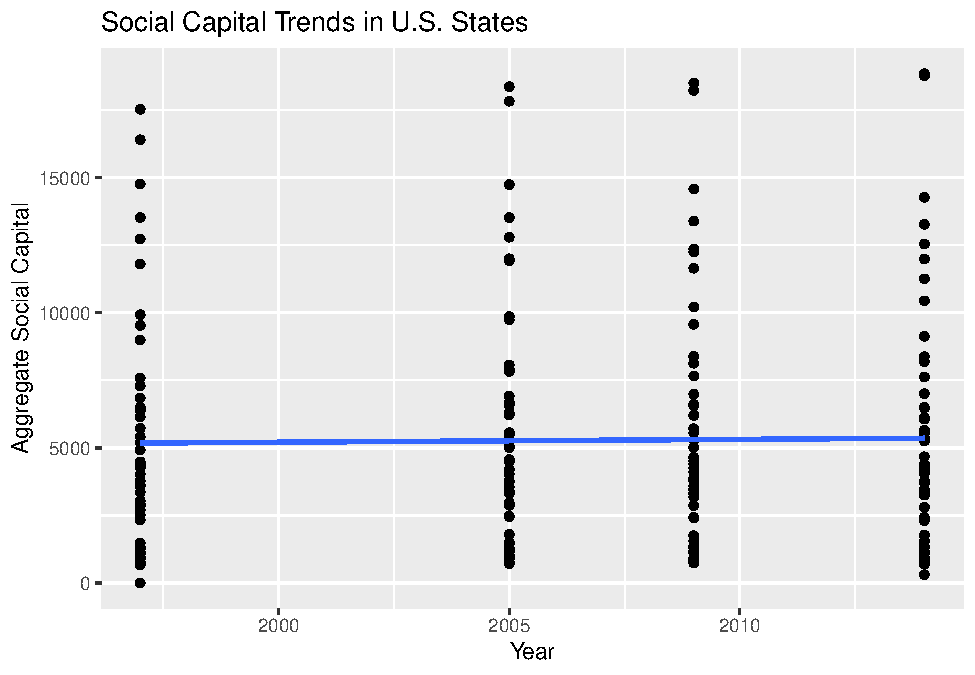
\includegraphics{Script_files/figure-latex/unnamed-chunk-1-1.pdf} 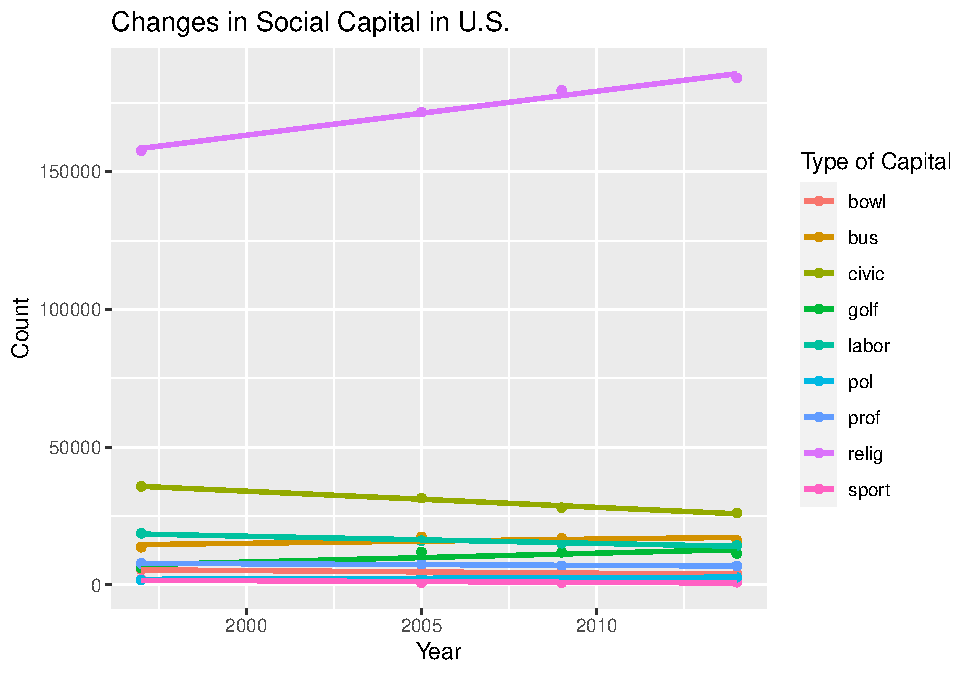
\includegraphics{Script_files/figure-latex/unnamed-chunk-1-2.pdf} 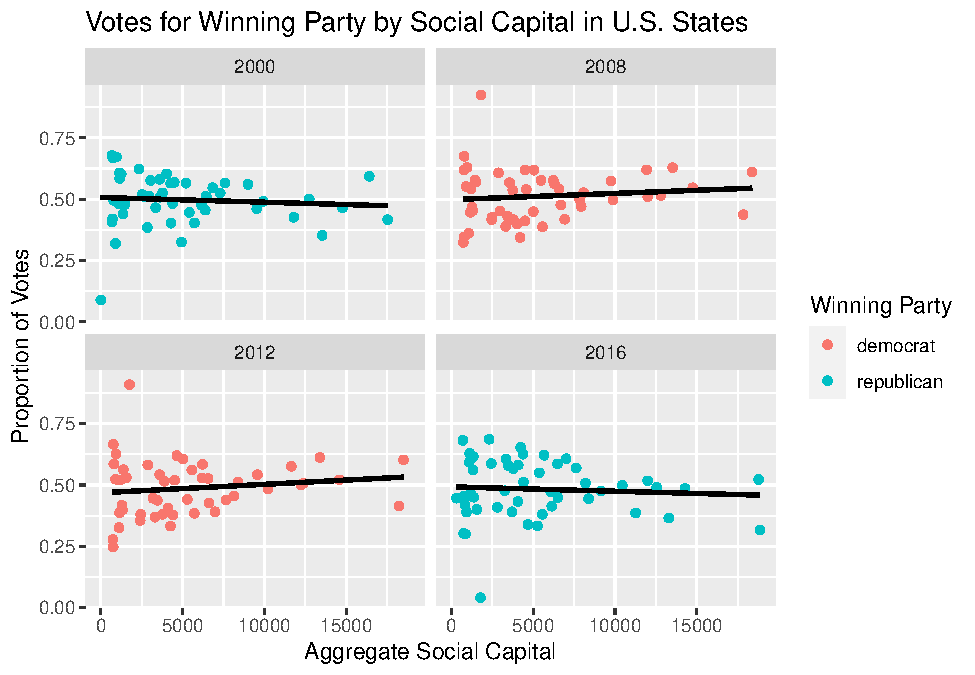
\includegraphics{Script_files/figure-latex/unnamed-chunk-1-3.pdf}

\begin{verbatim}
## Warning: package 'usmap' was built under R version 3.6.3
\end{verbatim}

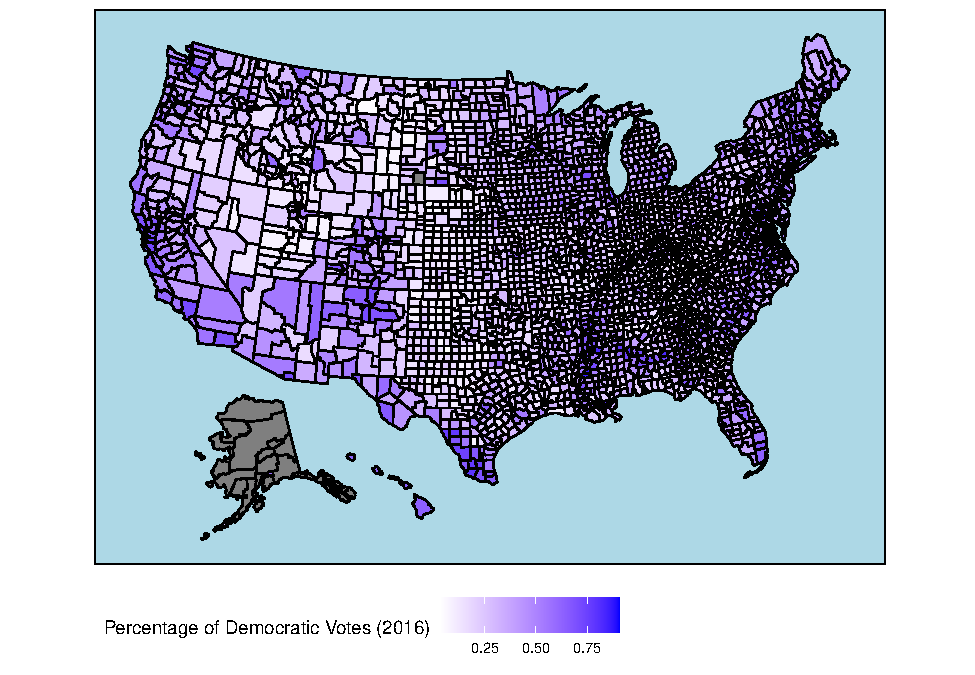
\includegraphics{Script_files/figure-latex/visualization part 2-1.pdf} 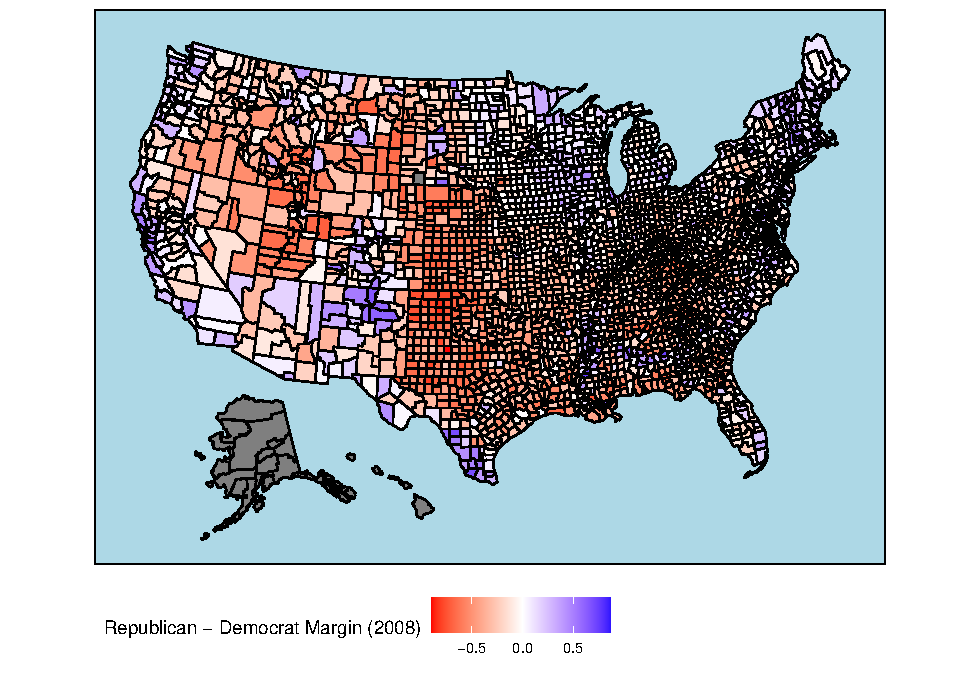
\includegraphics{Script_files/figure-latex/visualization part 2-2.pdf}

\begin{verbatim}
## [1] 2000 2008 2012 2016
\end{verbatim}

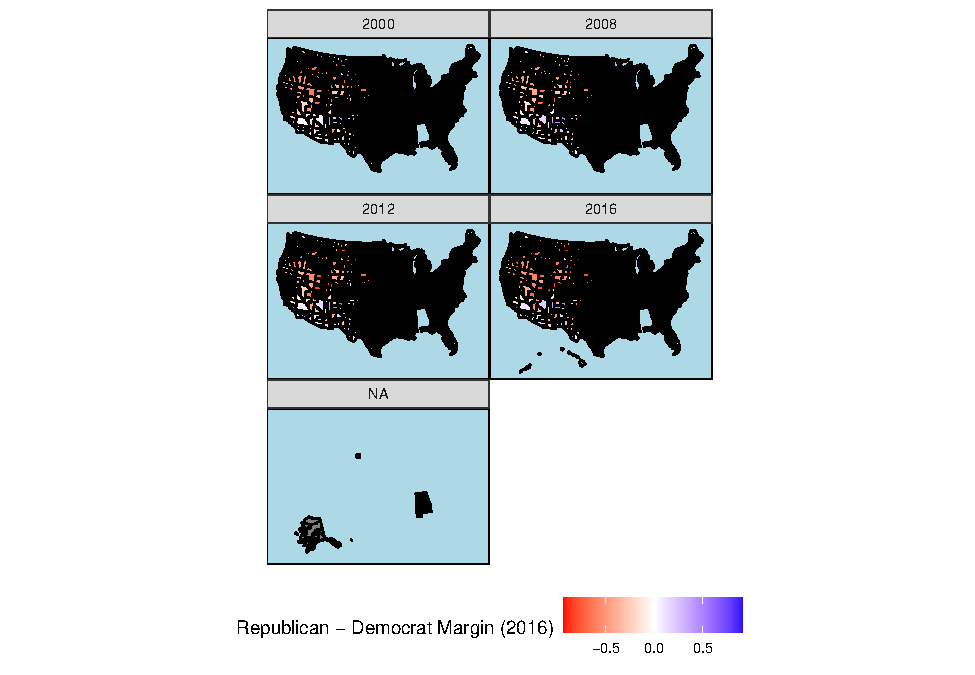
\includegraphics{Script_files/figure-latex/visualization part 2-3.pdf} 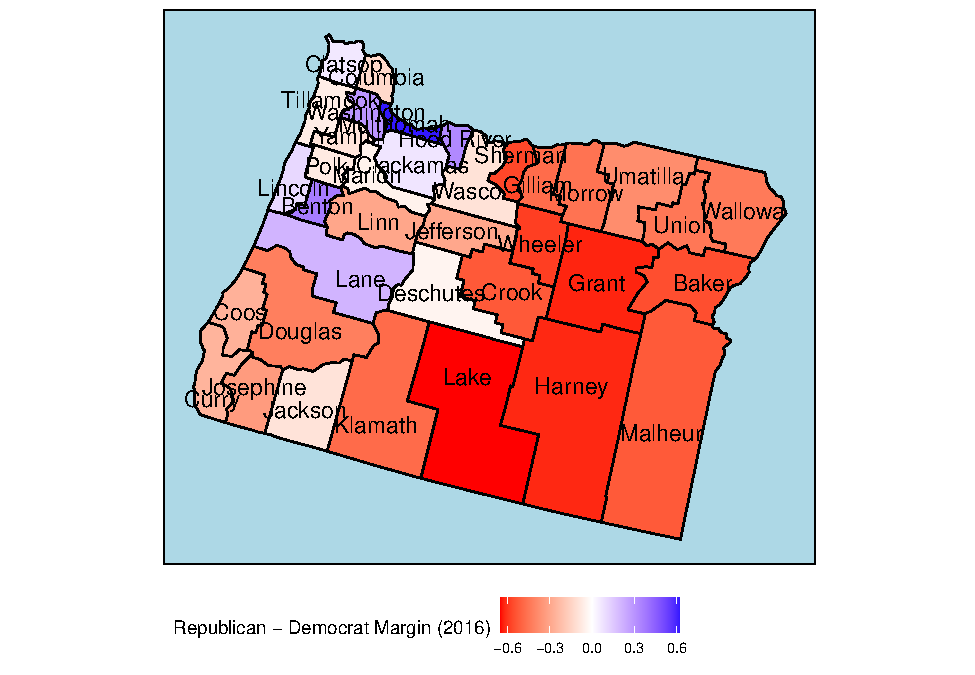
\includegraphics{Script_files/figure-latex/visualization part 2-4.pdf} 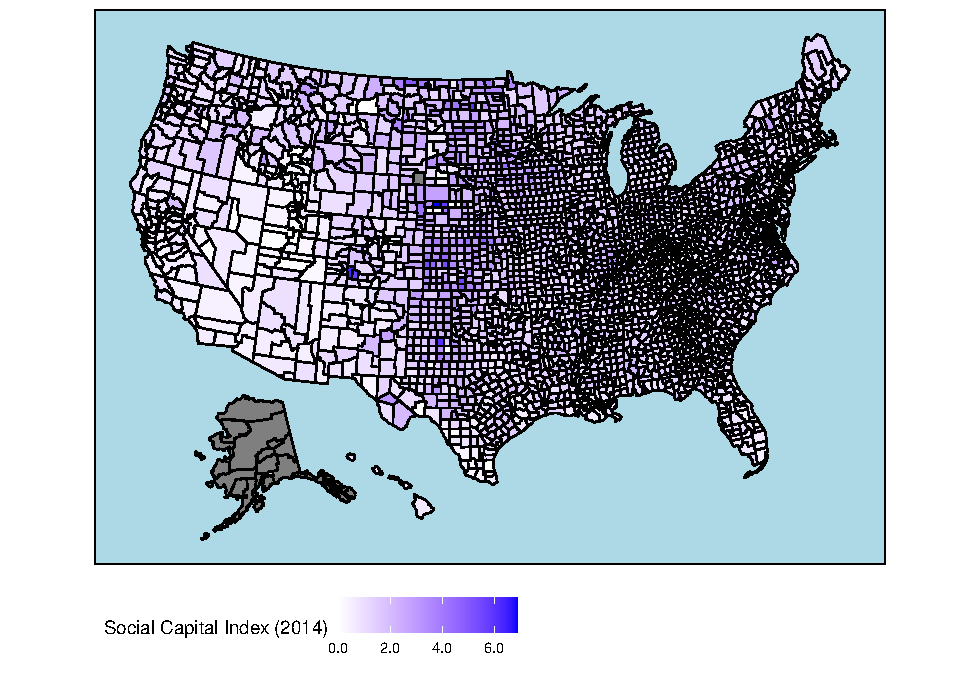
\includegraphics{Script_files/figure-latex/visualization part 2-5.pdf} 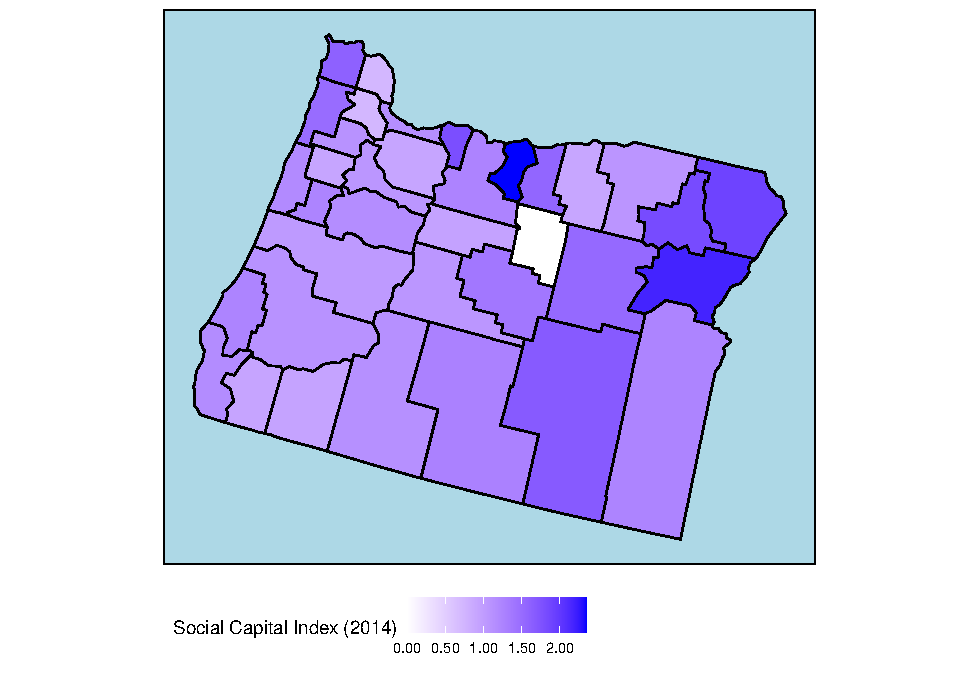
\includegraphics{Script_files/figure-latex/visualization part 2-6.pdf}

\hypertarget{results}{%
\section{Results}\label{results}}

\hypertarget{discussion}{%
\section{Discussion}\label{discussion}}

\newpage

\hypertarget{references}{%
\section{References}\label{references}}

We used R \autocite[Version 3.6.1;][]{R-base} and the R-packages \emph{dplyr} \autocite[Version 1.0.0;][]{R-dplyr}, \emph{forcats} \autocite[Version 0.5.0;][]{R-forcats}, \emph{ggplot2} \autocite[Version 3.3.2;][]{R-ggplot2}, \emph{here} \autocite[Version 0.1;][]{R-here}, \emph{janitor} \autocite[Version 2.0.1;][]{R-janitor}, \emph{kableExtra} \autocite[Version 1.3.1;][]{R-kableExtra}, \emph{knitr} \autocite[Version 1.29;][]{R-knitr}, \emph{magrittr} \autocite[Version 1.5;][]{R-magrittr}, \emph{papaja} \autocite[Version 0.1.0.9997;][]{R-papaja}, \emph{purrr} \autocite[Version 0.3.4;][]{R-purrr}, \emph{readr} \autocite[Version 1.3.1;][]{R-readr}, \emph{rio} \autocite[Version 0.5.16;][]{R-rio}, \emph{stringr} \autocite[Version 1.4.0;][]{R-stringr}, \emph{tibble} \autocite[Version 3.0.2;][]{R-tibble}, \emph{tidyr} \autocite[Version 1.1.0;][]{R-tidyr}, and \emph{tidyverse} \autocite[Version 1.3.0;][]{R-tidyverse} for all our analyses.

\begingroup
\setlength{\parindent}{-0.5in}
\setlength{\leftskip}{0.5in}

\hypertarget{refs}{}
\begin{CSLReferences}{0}{0}
\end{CSLReferences}

\endgroup


\printbibliography

\end{document}
